\pdfminorversion 7
\pdfobjcompresslevel 3

\documentclass[a4paper]{article}
\special{papersize=210mm,297mm}
\usepackage[utf8]{inputenc}
\usepackage[T1]{fontenc}
\usepackage{cite}
\usepackage[francais]{babel}
\usepackage[bookmarks=false,colorlinks,linkcolor=blue]{hyperref}
\usepackage[top=3cm,bottom=2cm,left=3cm,right=2cm]{geometry}
\usepackage{graphicx}
\usepackage{wrapfig}
\usepackage{subfig}
\usepackage{eso-pic}
\usepackage{array}
\usepackage{color}
\usepackage{xcolor}
\usepackage{url}
\usepackage{listings}
\usepackage{eurosym}
\usepackage{url}
\usepackage{textcomp}
\usepackage{fancyhdr} 

\definecolor{lightgray}{gray}{0.9}

\title{Rapport de Stage, Licence Informatique 3\up{ème} Année}
\author{Rémy \textsc{EL-SIBAIE BESOGNET}}


\newcommand{\HRule}{\rule{\linewidth}{0.5mm}}


\begin{document}


\begin{titlepage}

\begin{center}


% Upper part of the page

\textsc{\LARGE Université Paris Sud}\\[1.5cm]

\textsc{\Large Rapport de stage}\\[0.5cm]

\textsc{\Large Licence 3 Informatique}\\[0.5cm]

% Title
\HRule \\[0.4cm]
{ \huge \bfseries OCaml et Combinatoire}\\[0.4cm]

\HRule \\[1.5cm]

% Author and supervisor
\begin{minipage}{0.4\textwidth}
\begin{flushleft} \large
\emph{Auteur:}\\
Rémy \textsc{EL SIBAÏE BESOGNET}
\end{flushleft}
\end{minipage}
\begin{minipage}{0.4\textwidth}
\begin{flushright} \large
\emph{Encadrant:} \\
Jean-Christophe \textsc{FILLIÂTRE}
\end{flushright}
\end{minipage}

\vfill

% Bottom of the page
{\large \today}

\end{center}

\end{titlepage}


~
\vfill

\begin{center}
\section*{Résumé}
\end{center}
En informatique, de nombreux problèmes de combinatoire tels que le problème des 
n-reines ou les problèmes de pavage de tuiles peuvent se formaliser d'une
façon commune :
La couverture exacte de matrice, soit EMC\footnote{Exact Matrix Covering}. 
Plusieurs algorithmes permettent alors 
de résoudre cette question et donc les problèmes ci-dessus de façon générique.

Dans ce travail, j'ai implémenté, en OCaml, deux algorithmes de
résolution du recouvrement exact de matrice ayant pour nom 
Zero-suppressed Binary Decision
Diagram et Dancing Links. 
Ensuite, j'ai apporté des méthodes 
simplifiant la modélisation des problèmes de combinatoire pour les ramener
à un probleme de type EMC. L'utilisateur peut par 
exemple utiliser un mini langage fourni pour décrire son problème. Pour finir, 
ce stage est une contribution au langage OCaml et 
en fera bénéficier sa communauté qui manquait cruellement d'outils de 
combinatoire dans les bibliothèques existantes.

\vfill




\newpage
\section*{Remerciements}

Je remercie tout d'abord mon encadrant Jean-Chistophe Filliâtre, pour sa 
pédagogie hors du commun, le temps qu'il a pu prendre pour suivre mon 
travail, répondre à mes nombreuses questions ainsi que me critiquer de façon 
positive ou négative.
Je remercie évidemment l'ensemble de l'équipe ProVal pour cette ambiance 
chaleureuse durant les moments de pause et l'entraide dont j'ai pu 
bénéficier de la part de ses différents membres. Tout particulièrement, je 
remercie Sylvain Conchon pour le cours de Programmation Fonctionnelle du
premier semestre qui m'a donné envie de faire ce stage et qui l'a rendu 
possible.

Merci également à Nicolas, Léon et Joël pour m'avoir supporté déjà deux mois. 
Ainsi qu'à Astrid, Jean Noël, Florence, Lénaïc et les Pacatiens.


\newpage
\tableofcontents
\newpage
\listoffigures

\newpage
\section{Présentation}


J'ai effectué ce stage dans le cadre de ma troisième année de Licence en 
Informatique, sous la direction de Jean-Christophe Filliâtre (Equipe ProVal, 
LRI, Université Paris Sud 11 et CNRS / INRIA Saclay - Île-de-France). L'équipe 
ProVal a pour objectif de présenter des outils permettant de démontrer la 
validité de programmes par rapport à un comportement attendu en utilisant des
méthodes formelles de preuve.
Ces outils sont en majorité dévelopés en langage OCaml. 

Le but de mon stage n'est donc pas concentré sur le c\oe ur de métier de 
l'équipe. Il correspond plutôt à une contribution au langage OCaml. 
Cette contribution
prend la forme d'une bibliothèque pour la combinatoire, apportant
des méthodes simples permettant de modéliser des problèmes de combinatoire
sous forme de matrice de contraintes. Elle inclut l'implémentation de 
deux algorithmes permettant de résoudre le problème de la couverture exacte de
matrice ainsi qu'un langage pour décrire les problèmes de pavage.


\section{Couverture Exacte de Matrices}

\subsection{Définition}

Résoudre le problème de recouvrement exact de matrice 
(ou EMC~\footnote{Exact Matrix Covering en Anglais}) revient,
partant d'une matrice de booléens donnée, à trouver un sous-ensemble de 
lignes de cette matrice tel qu'il n'y ait qu'un et un seul '1' (ou \emph{true}) 
par colonne.
On considère par exemple la matrice suivante de taille 4x5 avec les lignes
notées de '0' à '5' : 

\[
  \begin{array}{ c }
   0. \\
   1. \\
   2. \\
   3. \\
   4. \\
  \end{array}
\left(
  \begin{array}{ c c c c c }
   1 & 0 & 1 & 1 \\
   0 & 1 & 1 & 0 \\
   1 & 1 & 0 & 1 \\
   1 & 0 & 0 & 1 \\
   0 & 1 & 0 & 0
  \end{array} \right)
\]

Dans cette exemple, on vérifie que :

\begin{description}
\item[$ \{3, 4\} $] ne correspond pas à une solution du probleme (pas de 1 dans la 3\up{e} colonne)
\item[$ \{0, 4\} $] constitue bien une solution (un et un seul 1 par colonne)
\item[$ \{1, 3\} $] constitue une autre solution
\end{description}

Il faut comprendre que le problème EMC correspond en fait à une liste de 
contraintes. Le but est donc de choisir un ensemble de lignes qui satisfassent 
chaque contrainte une et une seule fois.
Ce problème est connu pour avoir une complexité importante. On pourra observer 
plus tard qu'il peut être résolu par \emph{backtracking}.


\subsection{Applications}

Résoudre EMC est finalement une forme de programmation par contrainte. 
Plusieurs problèmes peuvent donc être encodés dans EMC à 
condition de pouvoir les modéliser tels quels. Je donne ici quelques 
exemples.


\subsubsection{Pavage}
Un problème de pavage est la recherche du nombre de façon 
(ou d'au moins une façon) de recouvrir un
plateau de jeu avec des tuiles (c'est-à-dire des pièces) d'une taille et d'une
forme choisie. Ces problème s'encodent parfaitement dans un problème EMC
puisqu'on cherche généralement à recouvrir chaque case une et une 
seule fois. 
On prend le problème trivial suivant : \\


\emph{De combien de façon peut-on recouvrir un échiquier de taille 
$4\times4$ par des dominos ?}
\\

Ce problème est trivial puisqu'il existe une formule mathématique pour le 
résoudre. On en connaît donc facilement le nombre de solutions. 
Ici, on ne prend 
pas en compte la quantité de dominos que l'on peut poser ni les symétries 
éventuelles du problème. On construit alors la
matrice EMC correspondante. Une colonne de la matrice représente une case de 
l'échiquier et une ligne de cette même matrice représente une façon de poser 
une tuile. On numérote les cases de 0 à 15.

\begin{figure}[h]
\centering
\rowcolors{1}{lightgray}{lightgray}
\[
  \begin{array}{|c|c|c|c|}
		\hline
   	0 & 1 & 2 & 3 \\
		\hline
    4	& 5 & 6 & 7 \\
		\hline
   	8 & 9 & 10 & 11 \\
		\hline
   	12 & 13 & 14 & 15 \\
		\hline
\end{array}
	\textrm{ }
\begin{array}{ |c| }
	\hline
		\\
	\hline
    \\
	\hline
  \end{array}
	\textrm{ }
\begin{array}{ |c|c| }
	\hline
		& \\ 
	\hline
  \end{array}
\]
\caption{\label{chessboard4x4} Echiquier 4x4 et dominos}
\end{figure}

Par exemple, poser un domino horizontalement sur la case 0 donne la ligne
de matrice suivante : 

\[
  \begin{array}{ c c c c c c c c c c c c c c c c }
	1 & 1 & 0 & 0 & 0 & 0 & 0 & 0 & 0 & 0 & 0 & 0 & 0 & 0 & 0 & 0 
  \end{array}
\]

On continue l'opération pour chaque case et on ajoute la ligne correspondante
si la pièce peut être posée à cet endroit. 
Une fois que toutes les cases du plateau ont été testées pour chacune des pièces,
on obtient la matrice EMC résultat. On a bien modélisé un problème de pavage 
sous forme de problème EMC dont nous verrons les algorithmes de résolution par
la suite.

\subsubsection{Sudoku}

Il n'est pas indispensable de décrire à nouveau le principe du 
Sudoku~\cite{sudoku} qui est massivement connu. Mais une explication concernant
sa modélisation en EMC s'impose.
Pour les problèmes de pavage, la contrainte se situait au niveau des cases.Dans
le cas du Sudoku, mettre une valeur dans une case du quadrillage impose 
5 contraintes sur la valeur et l'espace : 
\begin{itemize}
\item la case (l'espace)
\item la ligne (la valeur)
\item la colonne (la valeur)
\item la cellule 3x3 (la valeur)
\end{itemize}


\begin{figure}[h]
\centering
\[
\begin{array}{|c|c|c||c|c|c||c|c|c|}
\hline
5 & 3 &   &   & 7 &   &  &   &    \\
\hline
6 &   &   & 1 & 9 & 5 &  &   &    \\
\hline
  & 9 & 8 &   &   &   &  & 6 &    \\
\hline
\hline
8 &   &   &   & 6 &   &   &   & 3 \\
\hline
4 &   &   & 8 &   & 3 &   &   & 1 \\
\hline
7 &   &   &   & 2 &   &   &   & 6 \\
\hline
\hline
  & 6 &   &   &   &   & 2 & 8 &   \\
\hline
  &   &   & 4 & 1 & 9 &   &   & 9 \\
\hline
  &   &   &   & 8 &   &   & 7 & 5 \\
\hline
\end{array}
\]
\caption{\label{sudoku} Sudoku exemple (source : \cite{sudoku})}
\end{figure}


Effectivement, une fois qu'un élément est mis dans une case, il utilise l'espace
de cette case et empêche n'importe quel élément de prendre sa position. 
Il empêche aussi qu'un élément de même \emph{valeur} soit mis dans 
sa colonne, sa ligne et sa cellule. 
Il faut donc représenter chacune de ces contraintes dans les lignes de 
la future matrice EMC. On calcule donc pour chaque contrainte, le nombre de
colonnes de EMC demandées. On va donc prendre cet exemple.


\begin{enumerate}
\item 81 cases dans un Sudoku
: 81 colonnes pour les cases
\item $ 9~\textrm{lignes} \times 9~\textrm{valeurs} = $ 
81 colonnes pour les lignes
\item $ 9~\textrm{colonnes} \times 9~\textrm{valeurs} = $ 
81 colonnes pour les colonnes
\item $ 9~\textrm{cellules} \times 9~\textrm{valeurs} = $
81 colonnes pour les cellules
\end{enumerate}

On obtient donc une matrice d'une largeur de $ 81 \times 4 = 324 $ colonnes. 
Dans notre exemple le cas où l'on ajoute un 4 à la 7\up{e} ligne, 8\up{e} 
colonne donnerait la ligne de matrice EMC représentée par le code OCaml 
suivant : 

\lstinputlisting[language=Caml]{../imports/setsudoku.ml}


\subsubsection{N-reines}

Les N-Reines (ou N-Queens) est un problème d'Informatique et de Mathématiques 
assez connu lui aussi. 
Le but est de placer \emph{n} reines d'échec sur un échiquier $ n \times n $ tel
qu'aucune de ces reines ne puisse attaquer une autre reine. On cherche,
dans notre cas, toutes les solutions.
La mise en place la plus connue est $ n = 8 $, où le nombre de solutions est 
92. 

On sent bien, ici aussi, que poser une reine sur l'échiquier dépend de
différentes contraintes. 

\begin{figure}[h]
\begin{center}
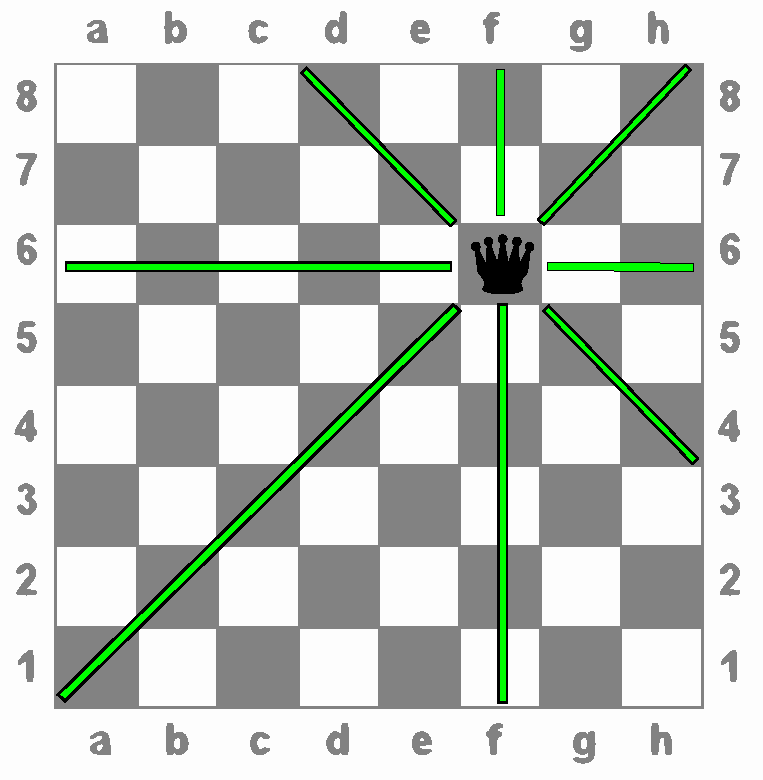
\includegraphics[height=0.2\textheight]{../imports/8queens.pdf}
\caption{\label{8queens} Poser une reine dans le problème des 8 reines}
\end{center}
\end{figure}

D'après la figure \ref{8queens}, on voit que les contraintes se font sur : 
\begin{itemize}
\item la ligne
\item la colonne
\item la diagonale gauche-droite
\item la diagonale droite-gauche
\end{itemize}

On peut éviter des considèrer les cases dans les contraintes : L'utilisation
d'une case est déjà comprise dans les quatres informations ci dessus (si une
reine utilise une ligne et une colonne choisie, alors elle utilise
forcément une seule case).
De plus, au lieu d'avoir une matrice dont la largeur 
(le nombre de colonne de EMC) est
quadratique en la taille du problème, avec cette représentation, elle est
linéaire.

On a : 
\begin{enumerate}
\item 8 lignes
\item 8 colonnes
\item 15 diagonales gauche-droite
\item 15 diagonales droite-gauche
\end{enumerate}

Ce qui correspond à une matrice de 46 colonnes (et non 64 si on avait choisis
les cases comme contrainte).
Cette façon de représenter le problème des N-Queens en EMC vient de Knuth, qu'il
décrit dans son article Dancing~Links~\cite{dlx} (que l'on verra plus loin). 
Un problème subsiste dans cette configuration. On remarque que jamais 8 reines
ne pourront recouvrir 15 diagonales. On ajoute alors le principe de colonnes 
secondaires. Ce sont des colonnes de la matrice EMC qui n'ont pas forcément
besoin de contenir un 1. Elle pourront alors contenir au maximum un 1.

Par exemple, si on place une reine en (a,8) (voir figure \ref{8queens}), on 
génère alors la ligne de matrice EMC représentée par le code OCaml suivant : 

\lstinputlisting[language=Caml]{../imports/setqueens.ml}


\section{Recherche des solutions}

Aucun des algorithmes existant ne peuvent résoudre EMC
avec une complexité polynomiale. Les seules solutions connues ne sont en fait
que de la force brute, et c'est souvent le cas en combinatoire.
Ceci étant, les deux méthodes implémentées durant ce stage sont 
très malines et très élégantes. C'est sans surprise puisque leur auteur est 
Donald E. Knuth.
Chacun de ces algorithmes possède ses avantages et ses inconvénients qu'il faut 
exploiter.

\subsection{L'algorithme Dancing Links}

The Dancing links~\footnote{Les liens dansants} ou DLX~\cite{dlx} 
est une implémentation efficace de l'algorithme X de Donald 
E. Knuth, proposée par lui-même dans son article éponyme. 
L'algorithme X est une solution pour résoudre 
les problèmes de couverture exacte de matrice vu plus haut.



\subsubsection{Principe de base et structure de donnée}

Avant d'entrer dans le vif du sujet, il faut commencer par l'astuce autour de 
laquelle tourne l'algorithme Dancing Links.
Partons d'une structure connue : la liste doublement chaînée.
N'importe quel programmeur saura ajouter un élément dans une liste doublement
chaînée.


\begin{figure}[h]
\begin{center}
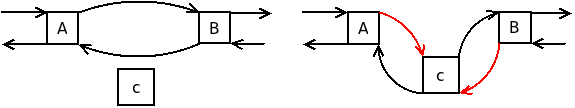
\includegraphics[scale=0.5]{../imports/add_elmt_dll.png}
\caption{\label{add_dll} Ajout d'un élément dans une liste doublement chaînée}
\end{center}
\end{figure}


Il suffit simplement de modifier quatres pointeurs comme indiqué 
figure~\ref{add_dll}. De même pour retirer un élément, il suffit de changer le 
pointeur de A vers C et le faire pointer vers B, et changer le pointeur de 
B vers C pour le faire pointer vers A. 

\begin{figure}[h]
\begin{center}
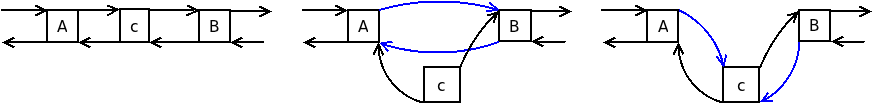
\includegraphics[scale=0.5]{../imports/delete.png}
\caption{\label{delete_dll} Suppression puis ré-ajout}
\end{center}
\end{figure}

On ne touche donc pas aux information de C. 
On peut donc connaître son ancienne position dans la liste. Si on veut
dans ce cas l'y remettre (Figure~\ref{delete_dll}), il suffit alors de modifier
à nouveau deux pointeurs
seulement : celui de Gauche[C] et celui de Droite[C] (donc de A et B).
Cette manipulation n'est pas courante mais elle convient parfaitement à 
l'algorithme X et elle est surtout très peu coûteuse.
Le nom poétique de cette algorithme vient de la manipulation astucieuse des 
pointeurs.

Maintenant que l'on connaît le principe, il faut comprendre comment il est
utilisé. Avant de faire tourner l'algorithme, nous devons génerer une structure
de donnée adaptée à partir de la matrice EMC. Cette structure (exotique) 
est une matrice construite à partir de listes doublement
 chaînées, c'est-à-dire une \emph{matrice doublement chaînée} que l'on appellera 
 matrice DLX. Cette dernière ne relie que les valeurs \emph{true} ou '1' de
 la matrice EMC.

\begin{figure}[h]
\begin{center}$
\begin{array}{c c}
\left(\begin{array}{ c c c c c }
   1 & 1 \\
   1 & 0 
  \end{array}\right) &
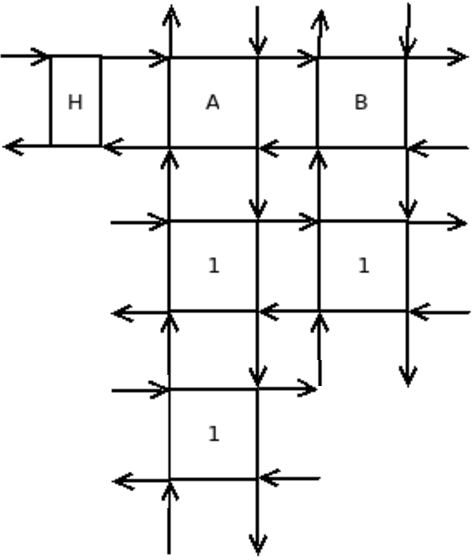
\includegraphics[scale=0.5]{../imports/dlx_matrice.pdf}
\end{array}$
\caption{\label{fig:gen_dlx}Création de la matrice DLX}
\end{center}
\end{figure}



Dans l'exemple~\ref{fig:gen_dlx}, on observe bien que seuls les '1' 
sont représentés.
De plus, la matrice DLX contient un en-tête général \emph{h} duquel l'algorithme
démarre le parcours ainsi qu'un en-tête par colonne.
Il faut évidemment bien faire attention au fait que la représentation est
cyclique et que le dernier élément d'une ligne pointe vers le premier et 
réciproquement (de même pour les colonnes). On peut définir cette structure en langage OCaml de la façon suivante : 
	
\lstinputlisting[language=Caml]{../imports/node.ml}



\subsubsection{Déroulement}

Pour résumer le déroulement de façon simple, on parcourt les colonnes au fur et
à mesure et pour chacune, on la recouvre elle et chacune 
des lignes 
où la colonne comporte un '1'. Puis on recommence jusqu'à ce que la matrice 
soit vide. Ensuite on retourne en arrière pour le backtracking. On decouvre 
donc la dernière colonne couverte puis on recommence. Et comme parfois, rien n'est plus explicite et clair qu'un morceau de OCaml, 
voici la fonction \emph{recherche} qui parcourt les solutions une par une et 
applique la fonction \emph{f} passée en paramètre :


\lstinputlisting[language=Caml]{../imports/search.ml}

Il suffit ensuite de passer à \emph{recherche} une fonction f permettant de
compter le nombre de solutions, ou qui les affiche.

\subsection{La structure Zero-Supressed Binary Decision Diagram}



Le ZSBDD, en français, Diagramme Binaire de décision avec suppression des zero, 
ou plus simplement ZDD, est une structure de donnée qui découle de BDD (Binary 
Decision Diagram). BDD est utilisé pour décrire une fonction booléenne. Un
BDD correspond à un graphe orienté acyclique (un arbre) dont les feuilles ont 
pour valeur
\emph{true} et \emph{false}. Les n\oe uds ont chacun deux fils et contiennent 
des variables booléennes. Le défaut de BDD dans les problèmes de combinatoire 
est que la majorité des 
champs finissent sur \emph{false} (ou $\bot$). C'est là qu'intervient le ZDD 
qui a simplement une interprétation différente d'un BDD. Grâce au ZDD on 
supprime environ 40\% des n\oe uds.
Cette structure est décrite par Donald E. Knuth dans 
The Art of Computer Programming \cite[p.249]{taocp4a}.

\subsubsection{Définition et construction}



Basiquement, un ZDD est un arbre binaire avec quelques propriétées : 

\begin{itemize}
\item Si un n\oe ud est une feuille alors sa valeur est $\bot$ (Bottom) ou 
$\top$ (Top)
\item S'il est à droite et que c'est une feuille alors sa valeur est $\top$
\item Sinon, il est étiqueté par un entier i, avec comme sous arbre droit 
$A_1$ et sous arbre gauche $A_2$ et se note : i $\rightarrow$ $A_1$, $A_2$ tel
que $A_1$ et $A_2$ ne contiennent pas d'élément j avec j $\leq$ i \\
\end{itemize} 

\begin{figure}[htp]
\begin{center}
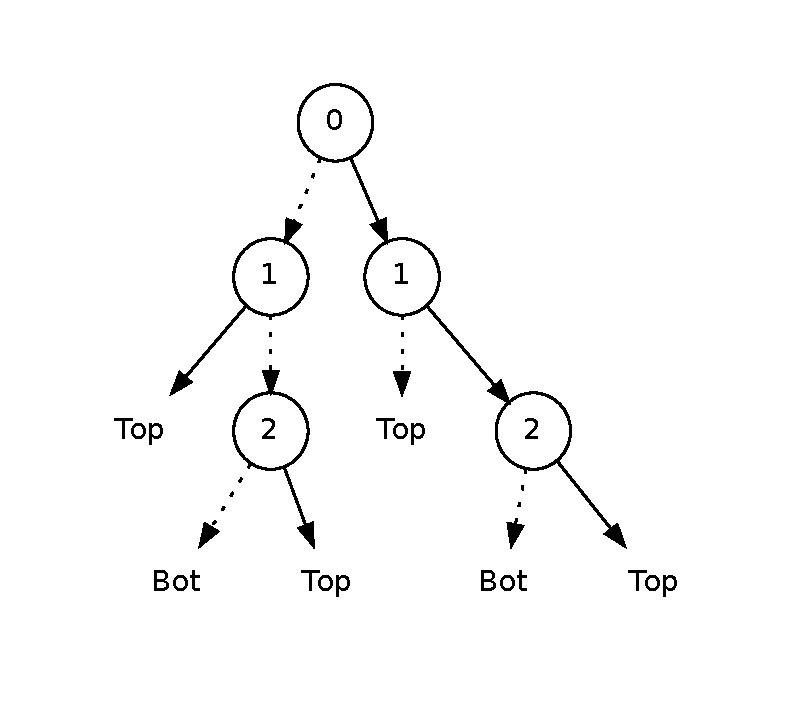
\includegraphics[scale=0.4]{../imports/zdd_ex.pdf}
\end{center}
\caption{\label{fig:zdd_exemple} Un exemple de ZDD}
\end{figure}

Une façon simple d'imaginer un ZDD est de le voir comme un ensemble d'ensembles 
d'entiers. 
On prend l'ensemble E = \{0, 1,...,n\}, $n \geq 1$. Un ZDD de E est une partie de 
l'ensemble 
des parties de E, soit un élément de P(P(E)). Le passage d'un ensemble à un ZDD
est bijectif. L'arbre gauche représente les ensembles ne contenant 
pas la valeur
\emph{i} courante. L'arbre droit correspond aux ensembles qui la contiennent.
L'ensemble représenté par un ZDD contient autant d'élément que le ZDD 
a de feuilles 
dont la valeur est $\top$.

On prend pour exemple le ZDD de la Figure \ref{fig:zdd_exemple}. Les traits en 
pointillés représentent les fils gauches et les traits pleins les fils droits.
Le moyen mnémotechnique pour obtenir l'ensemble représenté sur des 
exemples triviaux est de parcourir 
l'arbre de bas en haut à partir des $\top$. Quand on passe d'un n\oe ud fils à un n\oe ud père, si le fils était à droite
on ajoute le père à l'ensemble en construction, sinon on continue. 
Une fois sur le n\oe ud racine,
on recommence l'opération à partir d'une nouvelle feuille $\top$. Par exemple :

\begin{itemize}
\item $\top$ tout à gauche : $\top$ à droite : 1 y est 
$\rightarrow$ 1 à gauche : 0 n'y est pas.
On obtient l'ensemble \{1\}
\item $\top$ en bas à gauche : $\top$ à droite : 2 y est $\rightarrow$  
2 à gauche : 1 n'y est pas $\rightarrow$ 
1 à gauche : 0 n'y est pas. On obtient l'ensemble \{2\}
\item $\top$ milieu droite : $\top$ à gauche : 1 n'y est pas $\rightarrow$
1 à droite : 0 y est.
On obtient l'ensemble : \{0\}
\item $\top$ tout à droite : $\top$ à droite : 2 y est $\rightarrow$ 
2 à droite : 1 y est. $\rightarrow$ 
1 à droite : 0 y est. On obtient l'ensemble \{0, 1, 2\}
\end{itemize}

Ce ZDD est donc l'ensemble : \{\{0, 1, 2\}, \{0\}, \{1\}, \{2\}\}
On peut utiliser cette méthode pour effectuer l'opération inverse (obtenir
l'arbre depuis l'ensemble).


\subsubsection{Une structure optimisée}

Représenter un ZDD de taille immense demande forcément une place importante en 
mémoire. Cependant, en fonction du ZDD construit, de nombreux sous-arbres
peuvent parfois se répéter. Sachant que l'arbre se construit de façon récursive
, la méthode consiste à réutiliser les sous-
arbres déjà existants. 
Dans l'exemple de la Figure \ref{fig:zdd_exemple}, on peut donc reduire l'arbre
de la façon suivante : 
\begin{center}
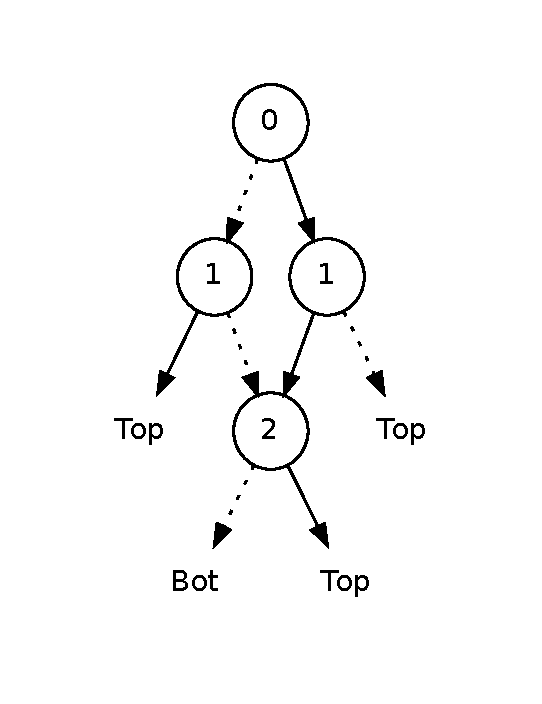
\includegraphics[scale=0.6]{../imports/zdd_construct.pdf}
\end{center}

Ceci est possible grâce au \emph{hash consing} qui est une
technique utilisée pour partager des valeurs structurellement égales. Ici,
les arbres sont stockés dans une table de hachage et au moment où un arbre est 
construit, on le cherche dans la table (en temps quasi-constant). S'il y est 
présent on le renvoie, sinon on le créé.

En OCaml, on utilise le type suivant pour représenter notre structure : 

\lstinputlisting[language=Caml]{../imports/zdd.ml}

A chaque ZDD, on attribut un identifiant unique quand il est calculé. On peut 
alors déterminer l'égalité de deux arbres de la façon suivante : 

$$egal(\top, \top) = true$$ 
$$egal(\bot, \bot) = true$$
$$egal((i1 \rightarrow R1, L1),(i2 \rightarrow R2, L2)  ) = (i1 = i2) 
\textrm{~et~}  (unique(R1) = unique(R2)) \textrm{~et~} (unique(R1) = unique(R2))
$$

De cette façon, on peut comparer deux ZDD en temps constant et savoir rapidement
si un arbre a déjà été construit ou non.

Avec ces outils optimisés on peut alors imaginer vouloir calculer le nombre de 
feuilles $\top$ et donc par la même occasion le cardinal de l'ensemble 
représenté par le ZDD. On utilise cette fois une technique qui utilise des
méthodes communes au \emph{hash consing} : la \emph{mémoïsation}. Le principe
est d'utiliser à nouveau une table de hachage pour aller stocker et récupérer
les résultats d'une fonction. 
En l'occurence, on créer donc une fonction \emph{cardinal} qui vérifie si le 
cardinal
de l'arbre passé en paramètre est dans la table. Si c'est le cas, il le renvoie
, sinon il le calcule et l'ajoute.
On peut, de cette façon, calculer des valeurs gargantuesques, très rapidement. 

\subsubsection{Utilisation pour EMC}

Les solutions de EMC sont des ensembles de lignes de la matrice. Si on 
représente les lignes par leur numéro, on a des ensembles d'entiers.
Rechercher l'ensemble des solutions d'un problème EMC revient donc à chercher 
un ensemble d'ensemble d'entiers, c'est à dire un ZDD. Pour commencer, 
observons ce problème sur une matrice EMC de taille 1x3 : 

\[
  \begin{array}{ c }
   0. \\
   1. \\
   2. \\
  \end{array}
\left(
  \begin{array}{ c }
   1 \\
   0 \\
   1
  \end{array} \right)
\]

Ici on observe facilement qu'il y a quatre solutions  : \{0\}, \{2\},
\{0, 1\} et  \{2, 1\}.
On doit donc construire le ZDD correspondant à l'ensemble \{\{0\}, \{2\}, 
\{0, 1\}, \{2, 1\}\}. 

\begin{center}
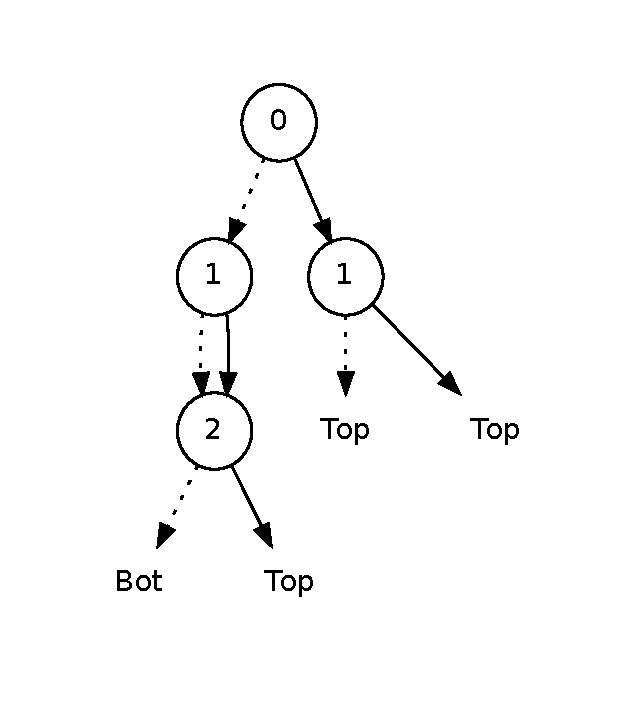
\includegraphics[scale=0.6]{../imports/zdd_sol_1x3.pdf}
\end{center}


La résolution est simple puisqu'il n'y a qu'une seule petite colonne. 
Passons maintenant à un problème autrement plus compliqué en utilisant la 
matrice EMC de la partie 1. 


\[
  \begin{array}{ c }
   0. \\
   1. \\
   2. \\
   3. \\
   4. \\
  \end{array}
\left(
  \begin{array}{ c c c c c }
   1 & 0 & 1 & 1 \\
   0 & 1 & 1 & 0 \\
   1 & 1 & 0 & 1 \\
   1 & 0 & 0 & 1 \\
   0 & 1 & 0 & 0
  \end{array} \right)
\]

On remarque que dans l'exemple précédent, on obtenait tous les ensembles pour
une colonne. Cette fois on veut les ensembles respectant les contraintes pour
la colonne 0, mais aussi la colonne 1 etc. On calcule donc séparément le ZDD
de chaque colonne, 
pour ensuite effectuer une intersection de tous ces arbres.
Par exemple pour la colonne 0, on obtient l'arbre suivant : 

\begin{center}
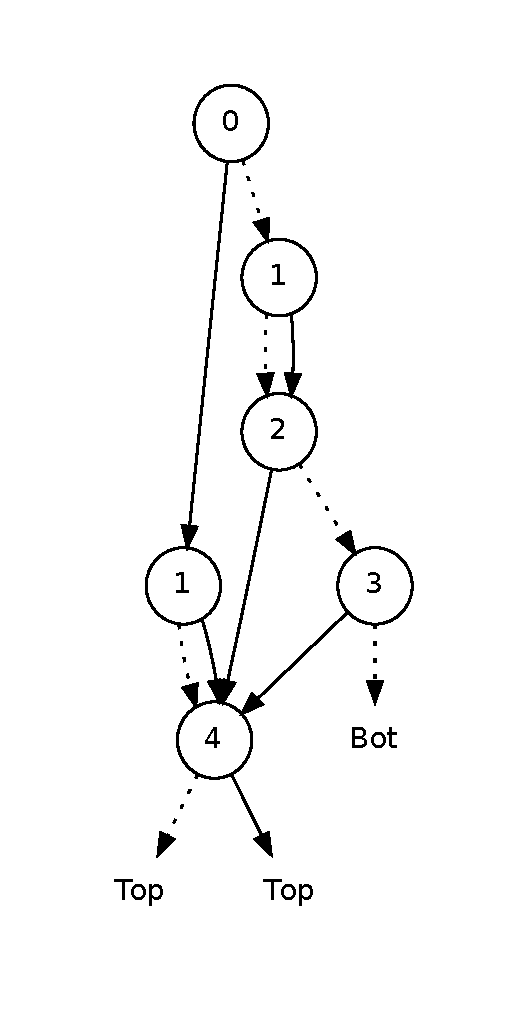
\includegraphics[scale=0.6]{../imports/column.pdf}
\end{center}

L'intersection peut être un procédé assez long à réaliser. L'utilisation 
du \emph{hash consing} est donc indispensable ici aussi. Dans la table, deux 
ZDD font office de clé et la valeur est le résultat de leur intersection.
Après avoir effectué l'intersection de tous les arbres on obtient : 


\begin{center}
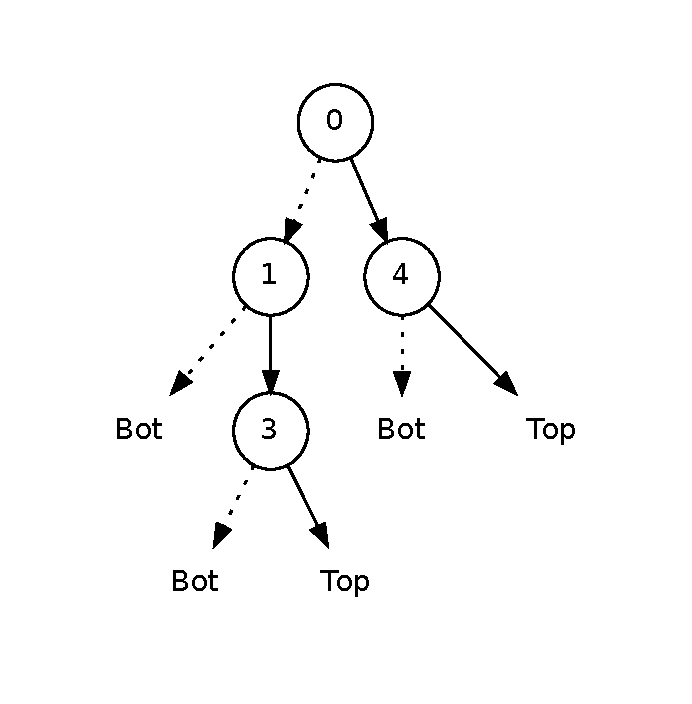
\includegraphics[scale=0.6]{../imports/inter.pdf}
\end{center}

Il ne reste plus ensuite qu'à appliquer la fonction \emph{cardinal} 
sur le ZDD resultat pour trouver le nombre de solutions. 

\subsection{ZDD vs DLX}

Maintenant que ZDD et DLX ont été décortiqués, il convient de les comparer.
Chacun a ses avantages et ses inconvenients :  


\paragraph{En temps}

: ZDD est l'algorithme le plus puissant des deux. Il peut
atteindre un nombre de solutions approchant la valeur $10^{23}$ en moins d'une 
dizaine de secondes. Pour la simple raison qu'il ne calcule pas les solutions
une par une, grâce à la \emph{memoïzation}. Cela semble évident quand on admet
grossièrement qu'un ordinateur "moyen" peut faire un milliard d'opérations par
seconde. DLX ne pourrait même pas atteindre cette valeur puisqu'il trouve les 
solutions une par une. C'est un algorithme de \emph{backtracking}.

Le soucis de ZDD est par contre la construction de l'arbre 
(c'est-à-dire l'intersection de tous les arbres des colonnes de EMC). 
Cette construction
est vraiment fonction de l'aspect de la matrice. Selon la façon dont cette 
dernière est formée, un même problème de pavage peut par exemple être 
résolu quasiment instantanément ou jamais. Effectivement, plus ZDD arrive à 
construire des sous arbre de taille croissante et plus il sera efficace.
ZDD dépend alors d'une heuristique
qui ordonne les colonnes de la matrice EMC dans un certain ordre 
avant de démarrer.
Cependant, une fois l'arbre construit, le calcul du nombre de solutions sera
toujours particulièrement rapide.
DLX est moins dépendant 
de la matrice EMC,
même si certaines heuristiques peuvent lui permettre d'optimiser sa vitesse.

\paragraph{En mémoire}

: DLX est le moins gourmand. DLX utilise simple une 
matrice doublement chaînée qui 
prend une très petite place en mémoire. Au contraire pour ZDD, son autre
défaut majeur est l'utilisation mémoire. Si la création ne se déroule 
pas de façon optimisée et que la matrice EMC n'a pas la bonne forme, 
la construction d'un ZDD peut 
utiliser jusqu'à plusieurs giga octets de mémoire pour un problème de pavage
un peu ardu. 

\paragraph{Quelques exemples}

: Sur le problème des N-Queens ou du Sudoku, DLX est très efficace 
puisqu'il atteint le rang 14 des N-Queens dans un temps assez correct 
(une quinzaine de secondes) et résoud un Sudoku à une solution instantanément. 
Au contraire, ZDD fait exploser l'utilisation
mémoire (sur la mâchine utilisée en stage) avant d'atteindre son but, dans les 
deux cas.

A l'inverse, ZDD bat à plate couture DLX dans les problèmes de pavage comme 
NxN-Dominos (recouvrire un échiquier de taille nxn avec des dominos) ainsi que
le problème de Knuth \cite[ex. 130, p252]{taocp4a} pour lequel il atteint le nombre 
hallucinant de 92.109.458.286.284.989.468.604 solutions (soit $\simeq 10^{23}$). 


\section{Une bibliothèque OCaml}

Durant ce stage, la mise en pratique de la théorie vue précédemment à été 
regroupée dans une 
bibliothèque OCaml ayant pour nom ReMl : Recouvrement Exact de Matrice en Ocaml.
Cette bibliothèque contient plusieurs outils permettant d'utiliser ZDD et DLX 
en modélisant différents problèmes encodés sous EMC.
Quelques exemples sont aussi fournis pour que l'utilisateur puisse s'en inspirer
.

\subsection{Architecture}

ReMl utilise tous les avantages du système de module d'OCaml. 

\begin{figure}[htp]
\begin{center}
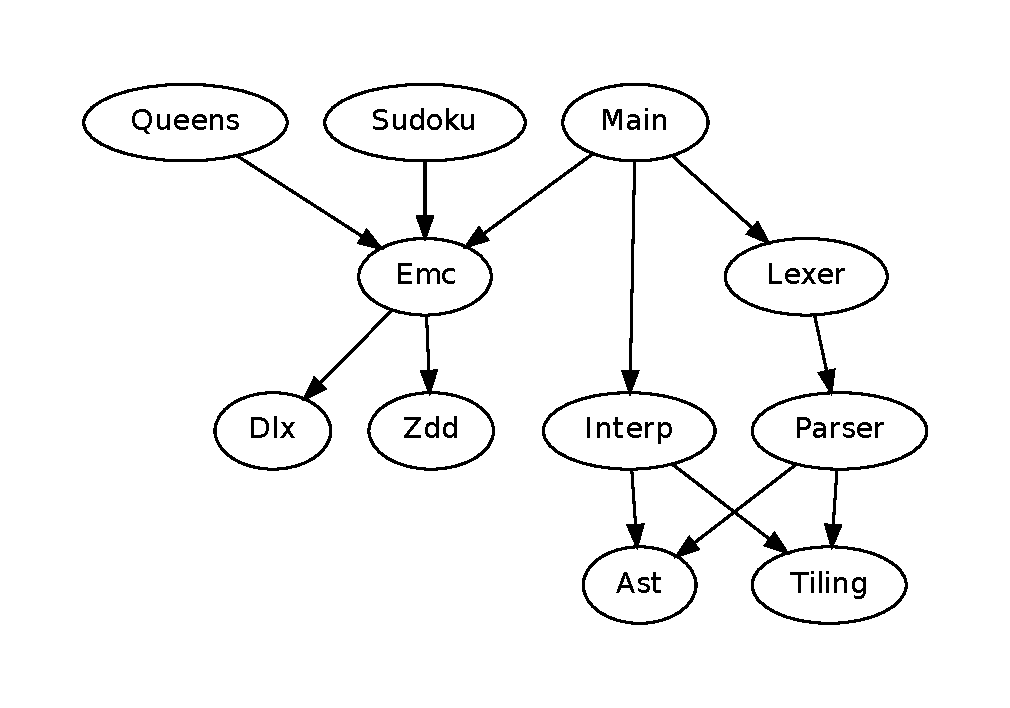
\includegraphics[scale=0.5]{../imports/archi.pdf}
\end{center}
\caption{\label{fig:archi} Architecture des modules de ReMl}
\end{figure}

L'implémentation de ZDD regroupe la plupart des opérations ensemblistes 
importantes et utilise la même interface que le module Set.S de OCaml. Il faut
cependant éviter certaines opérations qui ne seront pas efficaces avec cette 
structure. 
Dans le cas de Dlx, le module regroupe simplement l'algorithme ainsi que 
différentes façons de parcourir les solutions. Le module EMC est l'interface qui
utilise Zdd et Dlx et leur permet d'être indépendant des problèmes EMC.
Les modules Queens et Sudoku correspondent plutôt à une gallerie pour montrer
l'interêt et la puissance des algorithmes de Knuth. Ils utilisent évidemment la 
modélisation qui a été décrite dans la partie 1. 
Pour finir, une grosse partie de ce travail a été fournie dans le developpement
du module Tiling, permettant de modéliser les problèmes de pavage. Ce dernier
traîte différentes formes de tuiles à partir de matrices de booléens. 
Evidemment chacun de ces modules peut être utilisé à part entière.

\subsection{Un mini langage pour les problèmes de pavage}
Pour complèter le module de pavage et simplifier la description d'un problème, 
un mini-langage déclaratif a été créé. D'où la présence des
modules Parser, Lexer, Ast et Interp dans l'architecture. 
Ce langage permet de manipuler des tuiles sous forme de patrons (\emph{Pattern})
et de définir des variables de type problème prenant en paramètre des listes de 
patrons. Le langage est directement interprété et le module Main recherche 
alors les solutions pour chaque problème énoncé. 

On peut définir les patron de façon différentes : Soit directement avec le mot
clé \emph{constant} suivi de la taille et du remplissage par defaut des carrés,
soit en dessinant directement en ASCII entre 
\emph{\{\}}. Le caractère "\emph{*}" correspond à un carré plein et "\emph{.}" à
un carré vide.

\begin{figure}[h]
\centering
\begin{tabular}{c c}
\begin{lstlisting}
pattern b = {
**
.*
**
}
\end{lstlisting}&
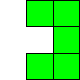
\includegraphics[scale=1]{../imports/patron.pdf}
\end{tabular}
\caption{le patron et la figure correspondante}
\label{fig:myfirsttable}
\end{figure}

L'exemple suivant permet par exemple de décrire le problème du pavage d'un 
échiquier de taille 8x8 par des dominos.

\lstinputlisting[language=Caml]{../imports/non-regression.rem}

On observe que dans la définition du problème, on passe une liste de pièces (qui
dans ce cas n'en contient qu'une), ainsi qu'une option "\emph{$\sim$sym}" qui 
signifie que l'on veut que toute les transformations de la pièce soient 
appliquées.
Par transformation, on entend les huits isométries du carré (les 8 isométries
qui laissent un carré invariant) : 

\begin{description}
\item[Les positives] : rotations 90°, 180°, 270° et Identité
\item[Les négatives] : Réflexion verticale, horizontale, par rapport aux 
première et deuxième diagonales
\end{description}
On ajoute alors dans la matrice EMC une ligne par position pour chaque 
transformation qui ne laisse pas la pièce invariante.
On peut aussi passer une option "\emph{$\sim$one}" ou "\emph{$\sim$maybe}" 
qui donne une information sur le dénombrement de
la pièce. En l'absence de cette option, on peut la poser de façon infinie.
Avec l'option, elle peut être posée une et une seule fois pour \emph{one}
et zero ou une fois pour \emph{maybe}.
Dans ce cas, on ajoute
une colonne à la matrice EMC qui ajoutera alors une contrainte sur la pose de 
la pièce.

Dans ce langage on peut aussi appliquer de nombreuses opérations sur les 
patrons, comme l'union, l'intersection ou la différence de deux patrons de même 
taille. L'utilisateur peut aussi s'il le souhaite appliquer un décalage,
insertion d'un patron constant dans un autre ou un changement de taille : 

\begin{lstlisting}
pattern b = {
**
.*
**
}

pattern c = resize b 5x5 		#changement de taille
pattern d = shift b 1x1			#decalage
\end{lstlisting}

Il est donc facile de résoudre un problème de pavage d'une dizaine de pièce,
comme les Pentaminos~\cite{pentamino}.

\newpage
\section{Conclusion}

Le travail principal de ce stage était donc d'effectuer une implémentation des
techniques existantes pour résoudre une famille de problèmes de combinatoire, à
savoir ceux encodables sous Exact Matrice Covering. Les résultats sont 
satisfaisant puisque les algorithmes implémentés donnent des réponses 
correctes dans un temps raisonnable. 
La facilité d'usage de ce programme en fait une 
contribution intéressante pour n'importe quel programmeur OCaml qui aimerait
traiter ce sujet. Cette bibliothèque apporte au langage de 
nombreux outils. Certains aspects mériteraient d'être implémentées pour 
aller plus loin : gestion 
des symétries du problème lui-même pour réduire le temps de calcul, amélioration
du mini-langage, etc. 
C'est donc ce qui m'attend dans la seconde partie de mon stage.

En conclusion, ce stage m'aura énormément appris. J'avais espérer travailler 
en OCaml et j'ai été très largement servi. En plus de connaître beaucoup
plus de détails et de structures intéressantes dans ce langage j'ai eu la 
chance de travailler en parallèle avec plusieurs paradigmes de programmation et
me renseigner grâce à de la littérature.
J'ai aussi eu la possibilité d'obtenir directement des conseils 
et des critiques 
sur le style de programmation et l'agorithmique. C'est finalement une chose qui
a manqué durant ma formation.
J'ai même eu le loisir d'orienter le sujet comme il me plaisait et ainsi 
approcher la compilation avec Menhir et ocamllex. 

Finalement j'ai 
découvert que le monde de la recherche en informatique m'attirait vraiment. 
J'ai pris beaucoup de plaisir à faire parti de l'équipe ProVal dont l'ambiance 
de travail est très agréable. Il me plairait, si j'en ai les possibilités, 
de postuler pour une thèse après mon Master.



\newpage
\addcontentsline{toc}{section}{\protect\numberline{}Bibliographie}
\bibliographystyle{plain}
\bibliography{./biblio}


\end{document}
